\documentclass[]{beamer}
% Class options include: notes, notesonly, handout, trans,
%                        hidesubsections, shadesubsections,
%                        inrow, blue, red, grey, brown

% Theme for beamer presentation.
\usepackage{beamerthemesplit} 
\usepackage{multimedia}
\usepackage{hyperref}

\usepackage{collectbox}

\usepackage[utf8]{inputenc}
\usepackage[english]{babel}

%%%%%%%%%%%%%%%%%%%%%%%%%%%%%%%%%%%%%%%%%%%%%%%%%%%%%%%%%%%%%%%%%%%%%%



\definecolor{mypink1}{rgb}{0.858, 0.188, 0.478}

\newcommand{\mybox}{%
    \collectbox{%
        \setlength{\fboxsep}{1pt}%
        \fbox{\BOXCONTENT}%
    }%
}

%%%%%%%%%%%%%%%%%%%%%%%%%%%%%%%%%%%%%%%%%%%%%%%%%%%%%%%%%%%%%%%%%%%%%%
% Other themes include: beamerthemebars, beamerthemelined, 
%                       beamerthemetree, beamerthemetreebars  

\title{PHY250: Harmonis Oscillations}    % Enter your title between curly braces
\author{Anabela R. Turlione}                 % Enter your name between curly braces
\institute{Digipen}      % Enter your institute name between curly braces
\date{Fall 2021}                    % Enter the date or \today between curly braces


\begin{document}

% Creates title page of slide show using above information
\begin{frame}
  \titlepage
\end{frame}
%\note{Talk for 30 minutes} % Add notes to yourself that will be displayed when
                           % typeset with the notes or notesonly class options

\section[]{}

% Creates table of contents slide incorporating
% all \section and \subsection commands
\begin{frame}
  \tableofcontents
\end{frame}


% \begin{frame}
%   % \centering
%    \movie[externalviewer]{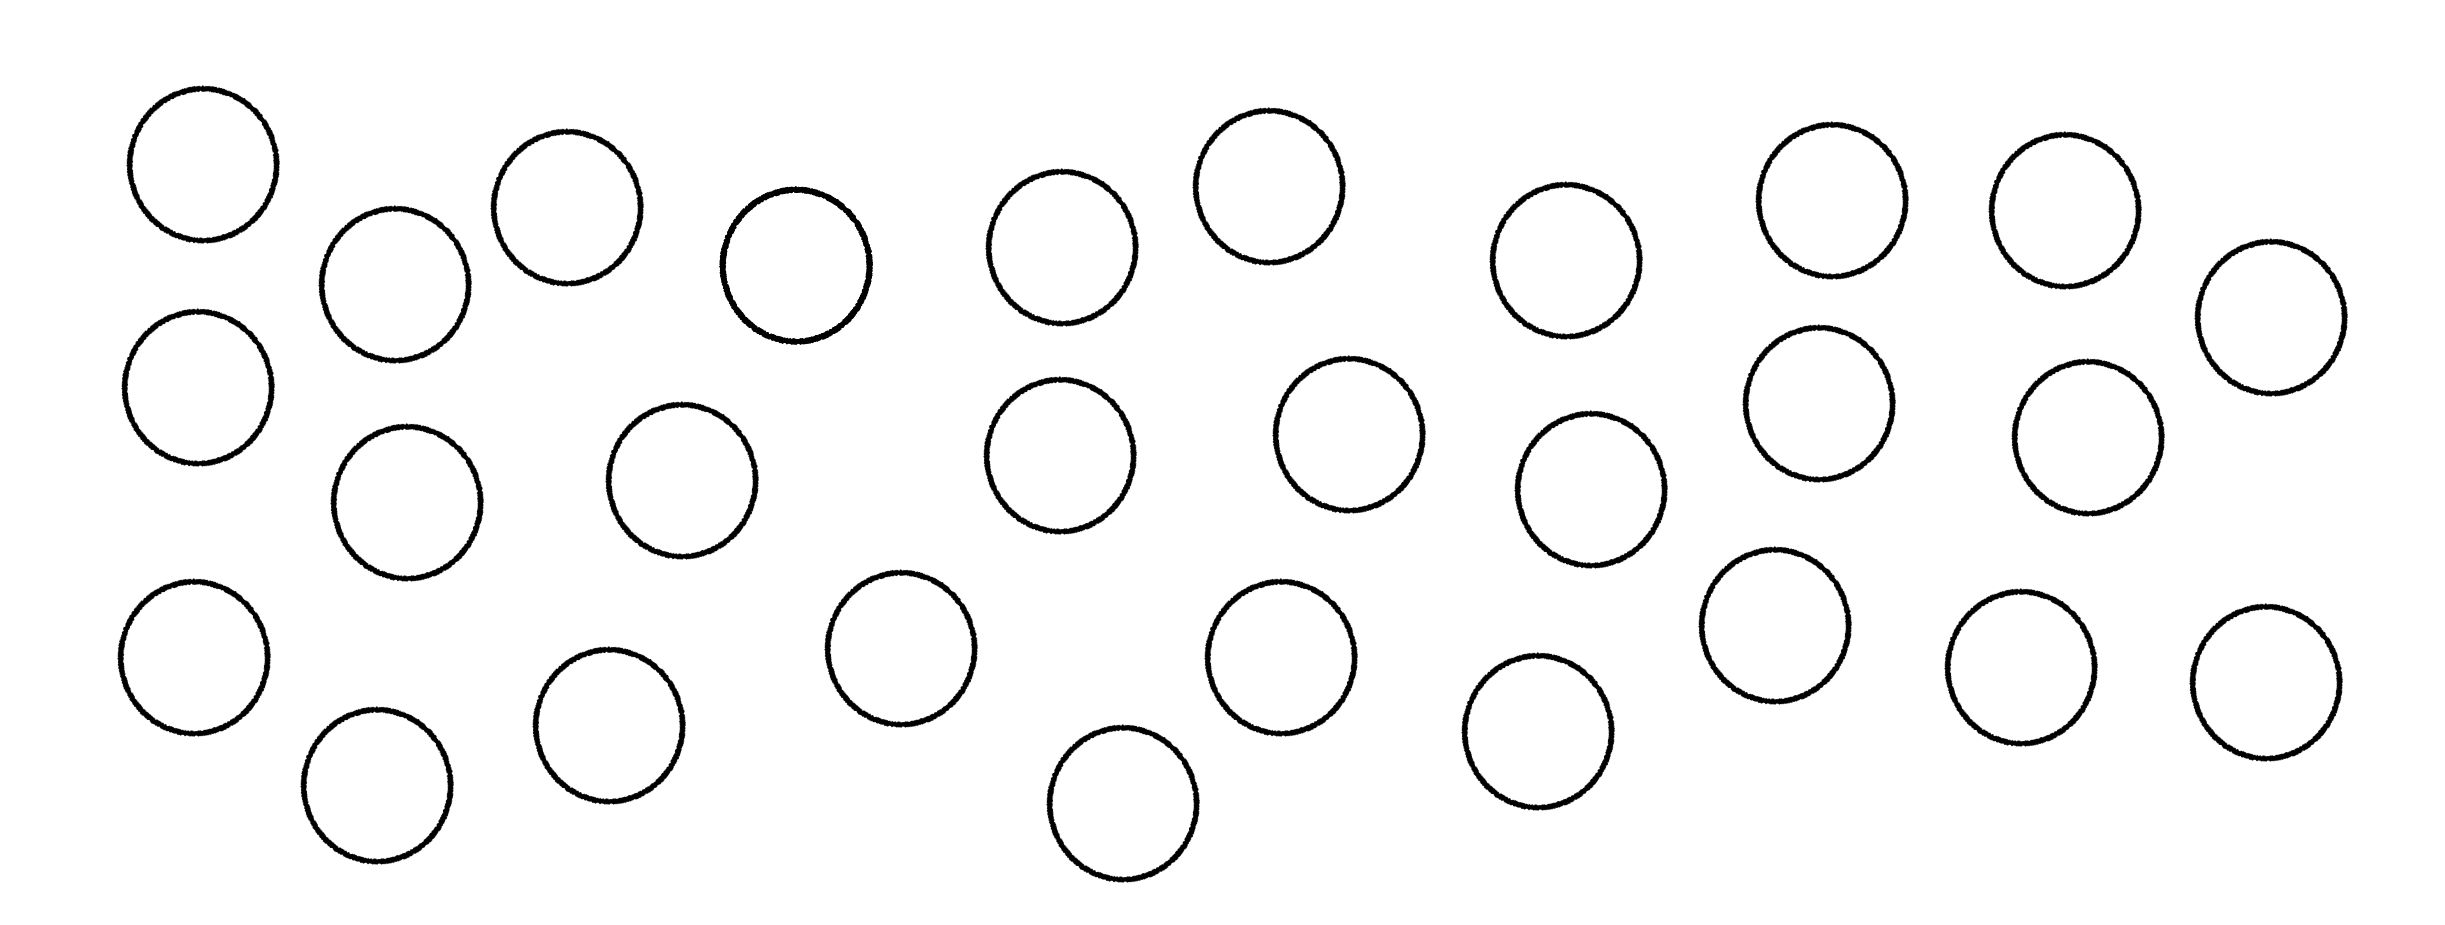
\includegraphics[width=\textheight ,
%    keepaspectratio]{surfacet1.jpg}}{test.mp4}

% \end{frame}
%%%%%%%%%%%%%%%%%%%%%%%%%%%%%%%%%%%%%%%%%%%%%%%%%%%%%%%%%%%%%%%%%%%

%%%%%%%%%%%%%%%%%%%%%%%%%%%%%%%%%%%%%%%%%%%%%%%%%%%%%%%%%%%%%%%%%%%
\section{Oscillations}
\subsection{The Harmonic Oscillator}

\begin{frame}
\frametitle{Simple Harmonic Motion}
Many objects vibrate or oscillate:
\vspace{3mm}

\begin{itemize}
\item An object at the end of a spring.
\item A tuning fork
\item The electric and Magnetic fields in the electromagnetic radiation.  
\item The atoms of a solid vibrate about their relatively fixed positions.
\item etc...
\end{itemize}
  


  \end{frame}

%%%%%%%%%%%%%%%%%%%%%%%%%%%%%%%%%%%%%%%%%%%%%%%%%%%%%%%%%%%%%%%


\begin{frame}
\frametitle{Simple Harmonic Motion}

Consider a system under the influence of a force proportional to the displacement 
\pause

\begin{equation}
 \vec{F}=-k\vec{\Delta x}~~~ \pause \textcolor{mypink1}{\leftarrow Hook's~Law}
\end{equation}  
\pause

This is the case of a mass on a spring: 


\begin{center}
  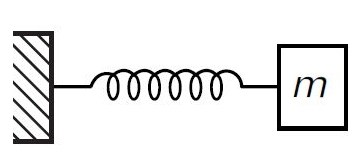
\includegraphics[height=1.in]{images3/spring0.jpg}
\end{center}


 \textcolor{mypink1}{higher}  the $k\pause\rightarrow$ the \textcolor{mypink1}{stiffer}  the spring.

  \end{frame}

  %%%%%%%%%%%%%%%%%%%%%%%%%%%%%%%%%%%%%%%%%%%%%%%%%%%%%%%%%%%%%%%


  \begin{frame}
    \frametitle{Simple Harmonic Motion}
    
    
    
      \begin{columns}[c]
       \column{2in}  % slides are 3in high by 5in wide
      
      \begin{center}
      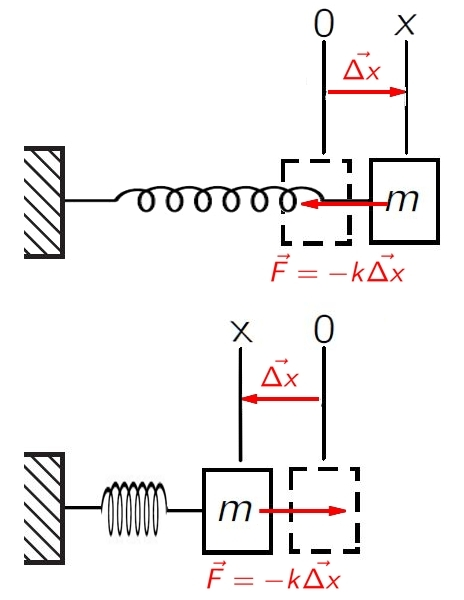
\includegraphics[height=2.in]{images3/springs.jpg}
    \end{center}
    
       \column{2.4in}
    \pause
    
 The force is a \textcolor{mypink1}{\textit{Restoring Force.}} 
    
       \end{columns}
    
      \end{frame}
  %%%%%%%%%%%%%%%%%%%%%%%%%%%%%%%%%%%%%%%%%%%%%%%%%%%%%%%%%%%%%%%

  %%%%%%%%%%%%%%%%%%%%%%%%%%%%%%%%%%%%%%%%%%%%%%%%%%%%%%%%%%%%%%%


\begin{frame}
  \frametitle{Simple Harmonic Motion}
  
  
  
    \begin{columns}[c]
     \column{2in}  % slides are 3in high by 5in wide
    
    \begin{center}
    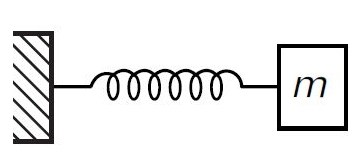
\includegraphics[height=1.in]{images3/spring0.jpg}
  \end{center}
  
     \column{2.4in}
 We are going to consider:
  
 \pause
  \begin{itemize}
  \item Massless spring.
  \pause
  \item The material of the spring in the elastic regime.
  \pause
  \item There are no friction or drag forces.
  \pause
  \item The coils are not close to touching.
  \end{itemize}
  
     \end{columns}
  
    \end{frame}
%%%%%%%%%%%%%%%%%%%%%%%%%%%%%%%%%%%%%%%%%%%%%%%%%%%%%%%%%%%%%%%

\begin{frame}
\frametitle{Simple Harmonic Motion}
What is the position $x$ as a function of the time?
\pause

\vspace{3mm}

In this case, the force is not constant, then  we can not use the results for a constant acceleration motion
\vspace{3mm}
\pause
\begin{equation*}
x\neq\frac{1}{2}at^2+v_ot+x_o
\end{equation*}  

To find the equations of motion for $x$, we use the second Newton's law:


\pause
\begin{eqnarray*}
\sum F&=&m a\\
-kx&=&m\frac{d^2x}{dt^2}\\
\end{eqnarray*} 

  \end{frame}

%%%%%%%%%%%%%%%%%%%%%%%%%%%%%%%%%%%%%%%%%%%%%%%%%%%%%%%%%%%%%%%


\begin{frame}
\frametitle{Simple Harmonic Motion}



we rearrange this to obtain,


\pause
\begin{equation}
\boxed{\frac{d^2x}{dt^2}+\frac{k}{m} x=0}
\label{eq:1}
\end{equation} 

\pause
\vspace{3mm}

 \textbf{Equation of motion for the simple harmonic oscillator}. 
\vspace{3mm}
\pause

\textcolor{mypink1}{How do we solve it?}

\vspace{3mm}
\pause
Trial solution: 

\vspace{3mm}

\pause

\begin{equation}
x(t)=Acos(\omega t+\phi)
\label{eq:2}
\end{equation}
%\pause

%Simple harmonic motion is thus always sinusoidal. Indeed, simple harmonic motion is defined as motion that is purely sinusoidal.

  \end{frame}

%%%%%%%%%%%%%%%%%%%%%%%%%%%%%%%%%%%%%%%%%%%%%%%%%%%%%%%%%%%%%%%


\begin{frame}
\frametitle{Simple Harmonic Motion}



If we put the trial solution \ref{eq:2} into the equation \ref{eq:1}, we obtain:

\pause
\begin{equation}
\boxed{\omega=\sqrt{\frac{k}{m}}}
\end{equation} 


\vspace{7mm}

\begin{itemize}
  \item Greater the mass $m\pause \rightarrow$ the lower the frequency $\omega$. \pause
  \item Stiffer the spring $k \pause\rightarrow$ the higher  $\omega$.
\end{itemize}






  \end{frame}



%%%%%%%%%%%%%%%%%%%%%%%%%%%%%%%%%%%%%%%%%%%%%%%%%%%%%%%%%%%%%%%


\begin{frame}
\frametitle{Simple Harmonic Motion}



 $x(t)$:periodic function

\pause

\begin{equation}
\rightarrow x(t)=x(t+T), \pause T=period
\end{equation}

\pause


\begin{equation}
  \rightarrow  Acos(\omega t+\phi)=Acos(\omega t+\omega T +\phi)
\end{equation}

\pause

\vspace{3mm}



\begin{equation}
  \rightarrow  \omega T=2\pi \pause\rightarrow \boxed{\omega=\frac{2\pi}{T}\pause }
\end{equation}



  \end{frame}

%%%%%%%%%%%%%%%%%%%%%%%%%%%%%%%%%%%%%%%%%%%%%%%%%%%%%%%%%%%%%%%%

\begin{frame}
  \frametitle{Simple Harmonic Motion}
  
  \begin{equation}
    \textcolor{mypink1}{\boxed{T}\pause   
    \rightarrow period,~~(units:s)}
  \end{equation}
  \pause
  \begin{equation}
    \textcolor{mypink1}{\boxed{\omega=\frac{2\pi}{T}}\pause   
    \rightarrow angular~frequency,~~(units:rad \cdot s^{-1 })}
  \end{equation}
\pause
 \begin{equation}
   \textcolor{mypink1}{\boxed{f=\frac{\omega}{2\pi}}\pause    \rightarrow frequency,~~(units: s^{-1 }= Hz)}
 \end{equation}


\end{frame}

%%%%%%%%%%%%%%%%%%%%%%%%%%%%%%%%%%%%%%%%%%%%%%%%%%%%%%%%%%%%%%%%




\begin{frame}
\frametitle{Simple Harmonic Motion}

\begin{equation*}
  x(t)= \textcolor{mypink1}{A}cos(\omega t+ \textcolor{mypink1}{\phi})
\end{equation*}

\pause

 \textcolor{mypink1}{what are $A$ and $\phi$?}


\pause
\begin{eqnarray*}
x(t=0)&=&x_0\\
\pause
v(t=0)&=&v_0\\
\\
\rightarrow Acos(\phi)&=&x_0\\
\pause
\rightarrow -A\omega sin(\phi)&=&v_0
\end{eqnarray*}
\pause



\begin{equation*}
 \left.
  \begin{array}{ll}
   \phi=tan^{-1}(\frac{v_0}{\omega x_0})\\
   A=\frac{x_0}{cos(\phi)}\\
  \end{array}
  \right\rbrace \pause~~ \textcolor{mypink1}{depend~~ on ~~the ~~initial~~ velocity ~~and ~~position}
  \end{equation*}


  \end{frame}



%%%%%%%%%%%%%%%%%%%%%%%%%%%%%%%%%%%%%%%%%%%%%%%%%%%%%%%%%%%%%%%



\begin{frame}
\frametitle{Simple Harmonic Motion}

For example, if $x(t=0)=x_0$ and $v(t=0)=0$,

\pause

\begin{eqnarray*}
v_0=-A\omega sin(\phi)=0\rightarrow \phi&=&n\pi,~n~integer\\
\\
 x_0=Acos(n\pi) \rightarrow A (-1)^n&=&x_0
\end{eqnarray*}

\pause

if $x_0>0$,  we can take $A>0$ and  $n=0$

\vspace{3mm}
\pause
Then,

\begin{equation*}
A=x_0
\end{equation*}
\pause
\begin{equation*}
\boxed{x(t)=A\cos\left(\sqrt{\frac{k}{m}}t\right)}
\end{equation*}


  \end{frame}



%%%%%%%%%%%%%%%%%%%%%%%%%%%%%%%%%%%%%%%%%%%%%%%%%%%%%%%%%%%%%%%



\begin{frame}
\frametitle{Simple Harmonic Motion}

if  $x(t=0)=0$ and $v(t=0)=v_0$, then

\pause

\begin{equation*}
Acos(\phi)=0\pause\rightarrow \phi=\boxed{\frac{(2n+1)}{2}\pi},~n~integer
\end{equation*}

\pause

\begin{equation*}
\rightarrow v_0=\pause-A \omega sin\Big(\frac{2n+1}{2}\pi\Big) \pause=\boxed{-A \omega (-1)^n}
\end{equation*}

\vspace{3mm}

\pause

if $v_0<0$,  we can take $A>0$ and  $n=0$. Then,

\pause

\begin{equation*}
A=-\frac{v_0}{\omega}
\end{equation*}

\pause

\begin{equation*}
x(t)=A\cos\left(\sqrt{\frac{k}{m}}t+\frac{\pi}{2}\right)\pause =\boxed{Asin\left(\sqrt{\frac{k}{m}}t\right)} 
\end{equation*}





  \end{frame}


%%%%%%%%%%%%%%%%%%%%%%%%%%%%%%%%%%%%%%%%%%%%%%%%%%%%%%%%%%%%%%%






\begin{frame}
\frametitle{Summarizing...}


For a Simple Harmonic Oscillator:

\begin{equation*}
x(t)=Acos(\omega t+\phi)
\end{equation*}

  \begin{center}
  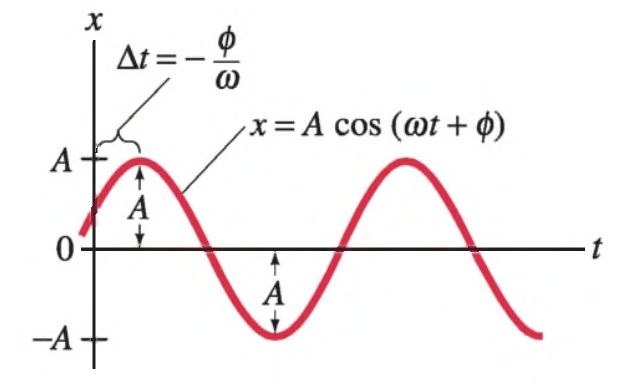
\includegraphics[height=1.7in]{images3/solution.jpg}
\end{center}


  \end{frame}





%%%%%%%%%%%%%%%%%%%%%%%%%%%%%%%%%%%%%%%%%%%%%%%%%%%%%%%%%%%%%%%


\begin{frame}
\frametitle{Summarizing...}




  \begin{center}
  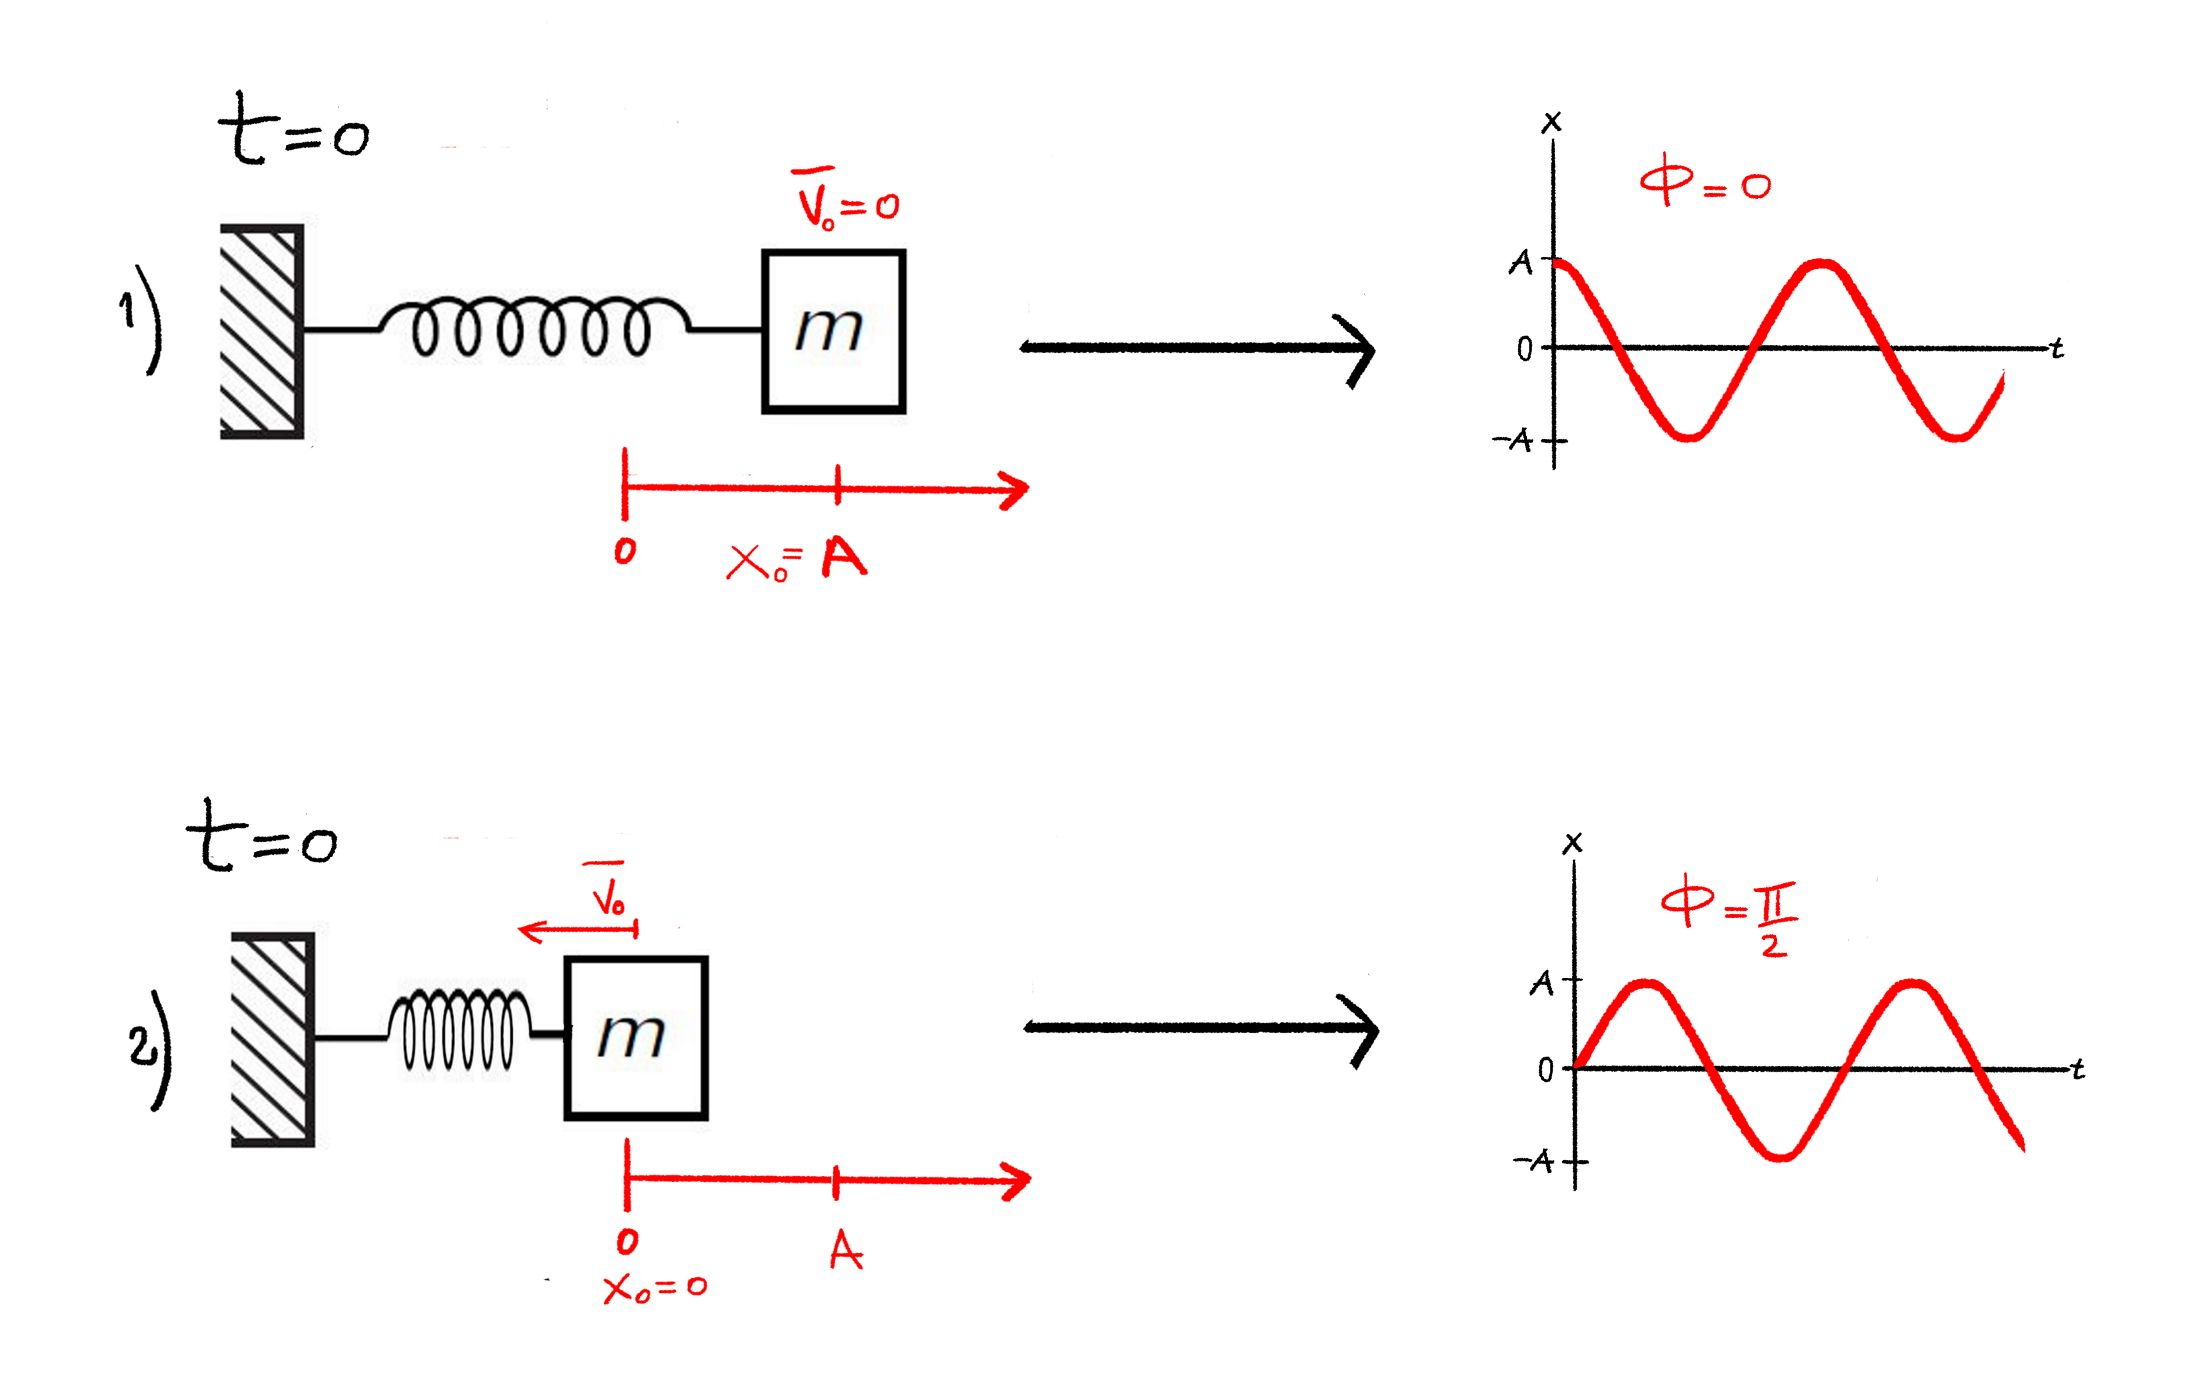
\includegraphics[height=2.8in]{images3/summarizing.jpg}
\end{center}


  \end{frame}


%%%%%%%%%%%%%%%%%%%%%%%%%%%%%%%%%%%%%%%%%%%%%%%%%%%%%%%%%%%%%%%

\begin{frame}
\frametitle{Summarizing...}




   \begin{columns}[c]
   \column{1.5in}  % slides are 3in high by 5in wide

\begin{equation*}
\phi=0 \rightarrow
\end{equation*}

   \column{2.5in}

    \begin{center}
  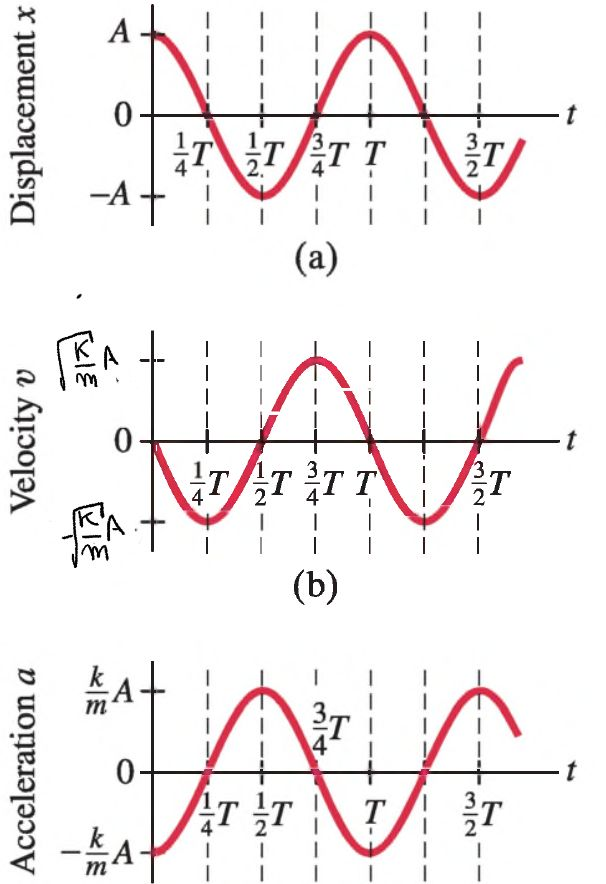
\includegraphics[height=2.8in]{images3/xva.jpg}
\end{center}


   \end{columns}




  \end{frame}
%%%%%%%%%%%%%%%%%%%%%%%%%%%%%%%%%%%%%%%%%%%%%%%%%%%%%%%%%%%%%%%


\begin{frame}
\frametitle{Simple Harmonic Motion}

We can write the solution in a different form:
\pause
\begin{equation*}
x(t)=A cos(\omega t +\phi)\pause = A cos (\phi)cos(\omega t)-A sin (\phi)sin(\omega t)
\end{equation*}
\pause

\textcolor{mypink1}{Rename the constants:}
\pause


\begin{eqnarray*}
Acos(\phi)&=&A'\\
Asin(\phi)&=&B'\\
\end{eqnarray*}

\pause

\begin{equation*}
\rightarrow x(t)=A' cos(\omega t)+B' sin(\omega t)
\end{equation*}

  \end{frame}

%%%%%%%%%%%%%%%%%%%%%%%%%%%%%%%%%%%%%%%%%%%%%%%%%%%%%%%%%%%%%%%

\begin{frame}
\frametitle{Simple Harmonic Motion Related
to Uniform Circular Motion}

    \begin{center}
  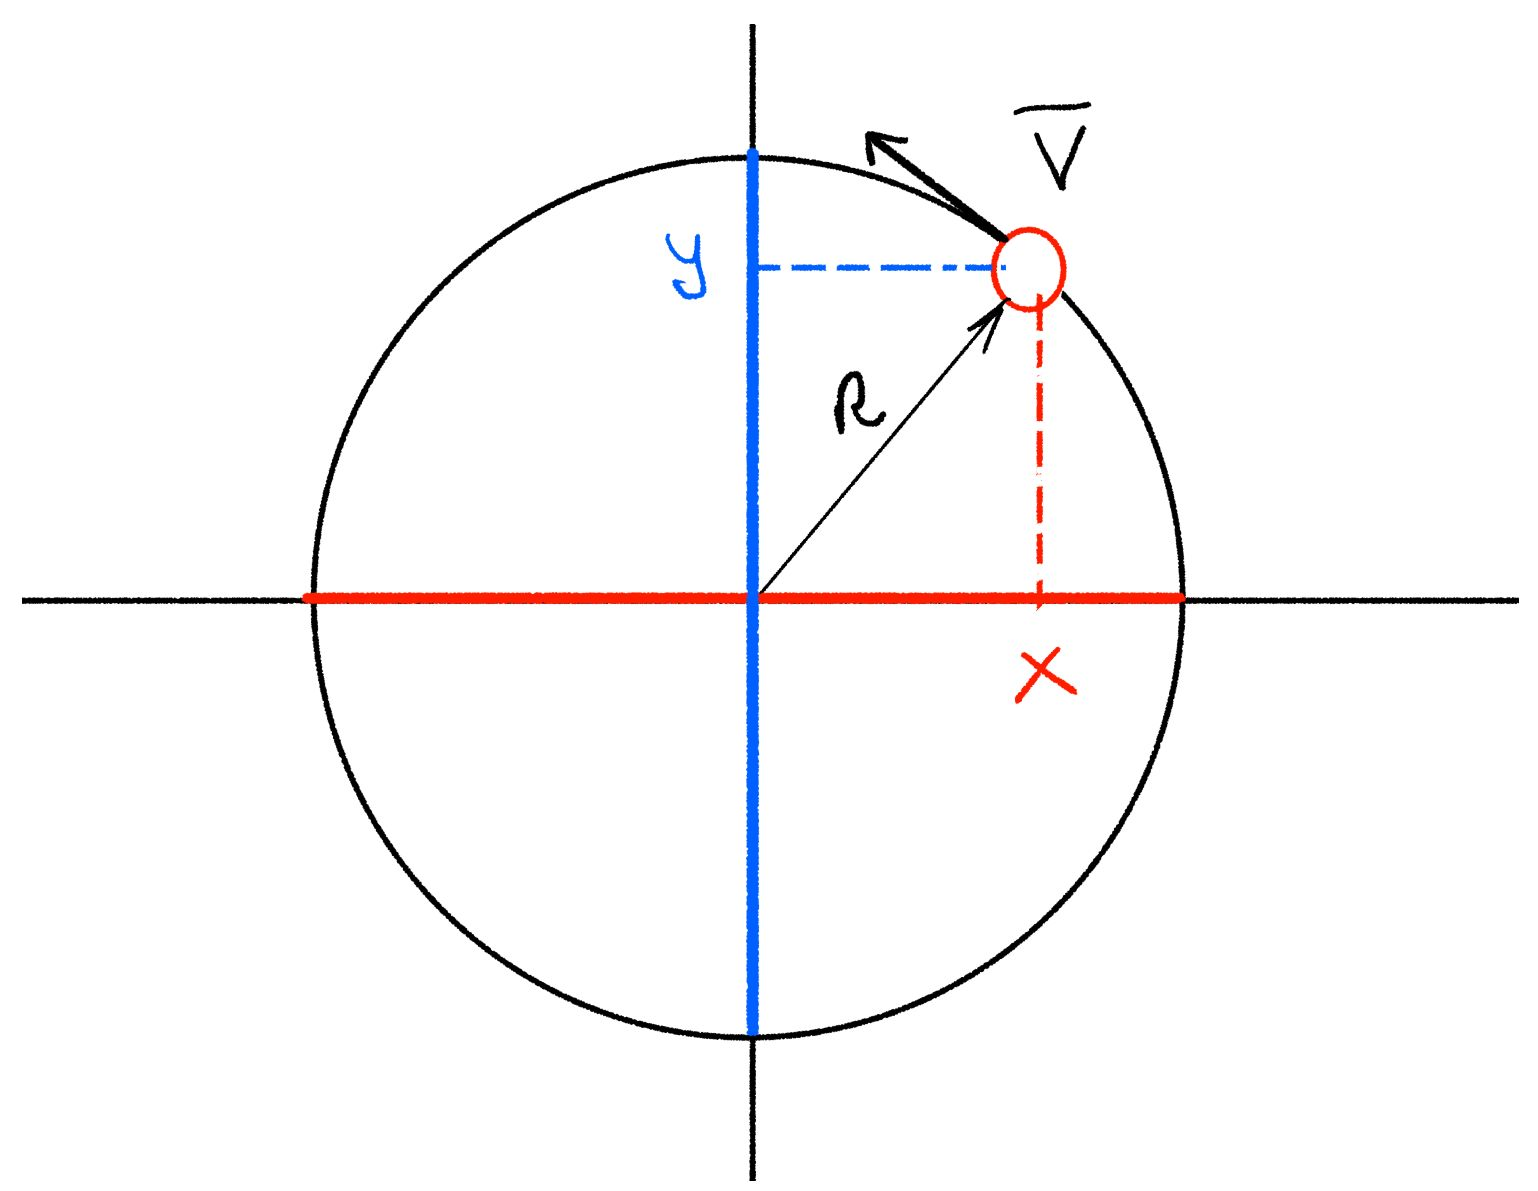
\includegraphics[height=1.2in]{images3/circular.jpg}
\end{center}


\begin{eqnarray*}
\vec{F}=-m\omega^2R\hat{r} \rightarrow F_x&=&-m\omega^2Rcos(\omega t +\phi)\\
F_y&=&-m\omega^2Rsin(\omega t +\phi)\\
\\
\pause
x=Rcos(\omega t +\phi) \rightarrow F_x&=&-m\omega^2x\\
y=Rsin(\omega t +\phi)  \rightarrow F_y&=&-m\omega^2y
\end{eqnarray*}


  \end{frame}

%%%%%%%%%%%%%%%%%%%%%%%%%%%%%%%%%%%%%%%%%%%%%%%%%%%%%%%%%%%%%%%

\begin{frame}
\frametitle{Simple Harmonic Motion Related
to Uniform Circular Motion}

We can analyze oscillatory
motion in a simpler way if we imagine it to be a projection of something
going in a circle.

\vspace{5mm}

If we do this, we will be able to
analyze our one-dimensional oscillator with circular motions, which is a lot easier
than having to solve a differential equation. The trick in doing this is to use
complex numbers.

\end{frame}

%%%%%%%%%%%%%%%%%%%%%%%%%%%%%%%%%%%%%%%%%%%%%%%%%%%%%%%%%%%%%%%

\begin{frame}
\frametitle{Generalization}

The  Simple Harmonic Oscillator equation is  a linear differential equation, 

\begin{equation*}
a_n\frac{d^nx}{dt^n}+a_{n-1}\frac{d^{n-1}x}{dt^{n-1}}+....+a_1\frac{dx}{dt}+a_ox=0
\end{equation*}

with $n=2$
\vspace{3mm}

The trial solution for this kind of equations is $x(t)=Ae^{\alpha t}$.

\vspace{3mm}

If we replace this solution in the case of the Harmonic Oscillator, we obtain the equivalent equation


\begin{equation*}
\alpha^2+\frac{k}{m}=0\rightarrow \alpha=\pm i\sqrt{\frac{k}{m}}=\pm i\omega 
\end{equation*}

\end{frame}

%%%%%%%%%%%%%%%%%%%%%%%%%%%%%%%%%%%%%%%%%%%%%%%%%%%%%%%%%%%%%%%

\begin{frame}
\frametitle{Generalization}

The, the general solution of the equation is,

\begin{equation}
x(t)=Ae^{i\omega t}+Be^{-i\omega t}
\end{equation}


Using the identity, $e^{i\omega t}=cos(\omega t)+i sin(\omega t)$ Rearranging it, we can obtain again the solution in terms of $cos$ and $sin$:



\begin{equation}
x(t)=A'cos(\omega t)+B' sin(\omega t)
\end{equation}




\end{frame}




%%%%%%%%%%%%%%%%%%%%%%%%%%%%%%%%%%%%%%%%%%%%%%%%%%%%%%%%%%%%%%%

\begin{frame}
\frametitle{Energy in the Simple Harmonic Oscillator}

The potential of a particle that has a Simple Harmonic motion is,
\pause
\begin{equation}
F=-kx\rightarrow U=-\int Fdx=\frac{1}{2}kx^2
\end{equation}
\pause
where we set $U(x=0)=0$.
\vspace{3mm}
\pause

Then the total mechanical energy of a  Simple Harmonic Oscillator is,
\pause
\begin{equation}
E=\frac{1}{2}mv^2+\frac{1}{2}kx^2
\end{equation}

\pause
If we use the expressions for $x$ and $v$,
\pause
\begin{equation}
E=\frac{1}{2}m{[A\omega sin(\omega t +\phi)]}^2+\frac{1}{2}k{[Acos(\omega t +\phi)]}^2
\end{equation}

\end{frame}



%%%%%%%%%%%%%%%%%%%%%%%%%%%%%%%%%%%%%%%%%%%%%%%%%%%%%%%%%%%%%%%

\begin{frame}
\frametitle{Energy in the Simple Harmonic Oscillator}



\begin{equation}
E=\frac{1}{2}kA^2{[ sin(\omega t +\phi)}^2+{cos(\omega t +\phi)]}^2=\frac{1}{2}kA^2
\end{equation}

\vspace{5mm}
\pause
    \begin{center}
  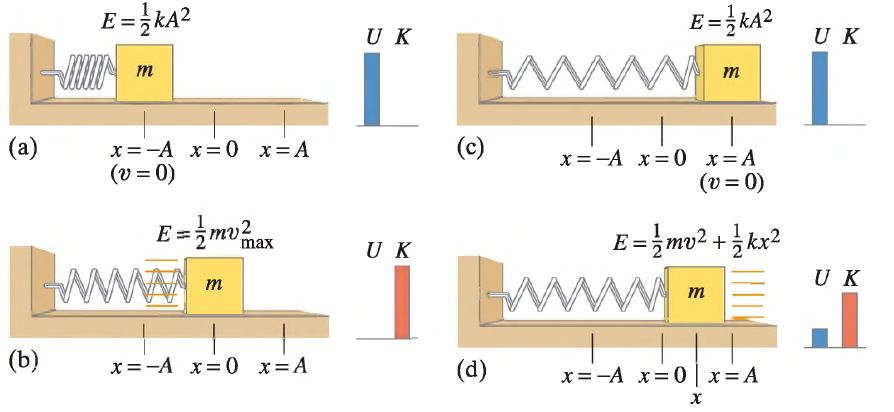
\includegraphics[height=1.8in]{images3/energy1.jpg}
\end{center}
\end{frame}




%%%%%%%%%%%%%%%%%%%%%%%%%%%%%%%%%%%%%%%%%%%%%%%%%%%%%%%%%%%%%%%

\begin{frame}
\frametitle{Energy in the Simple Harmonic Oscillator}



Potential Energy Graph

\vspace{5mm}

    \begin{center}
  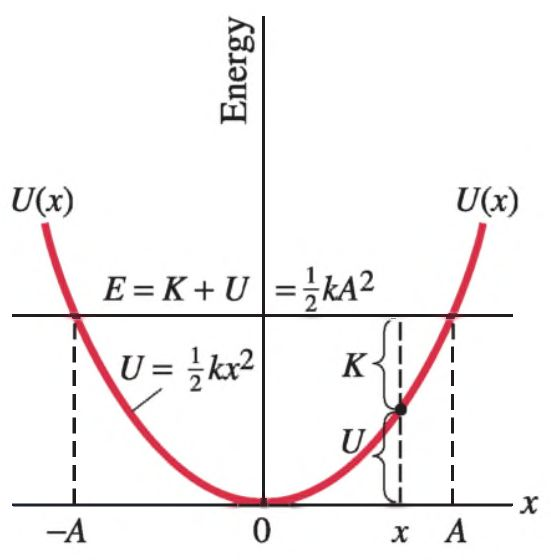
\includegraphics[height=2.2in]{images3/energy2.jpg}
\end{center}
\end{frame}


%%%%%%%%%%%%%%%%%%%%%%%%%%%%%%%%%%%%%%%%%%%%%%%%%%%%%%%%%%%%%%%

\begin{frame}
\frametitle{The Simple Pendulum}

For small displacements, the motion of a symple pendulum  is essentially simple harmonic.

\pause

   \begin{columns}[c]
   \column{2in}  % slides are 3in high by 5in wide
  


  \begin{center}
  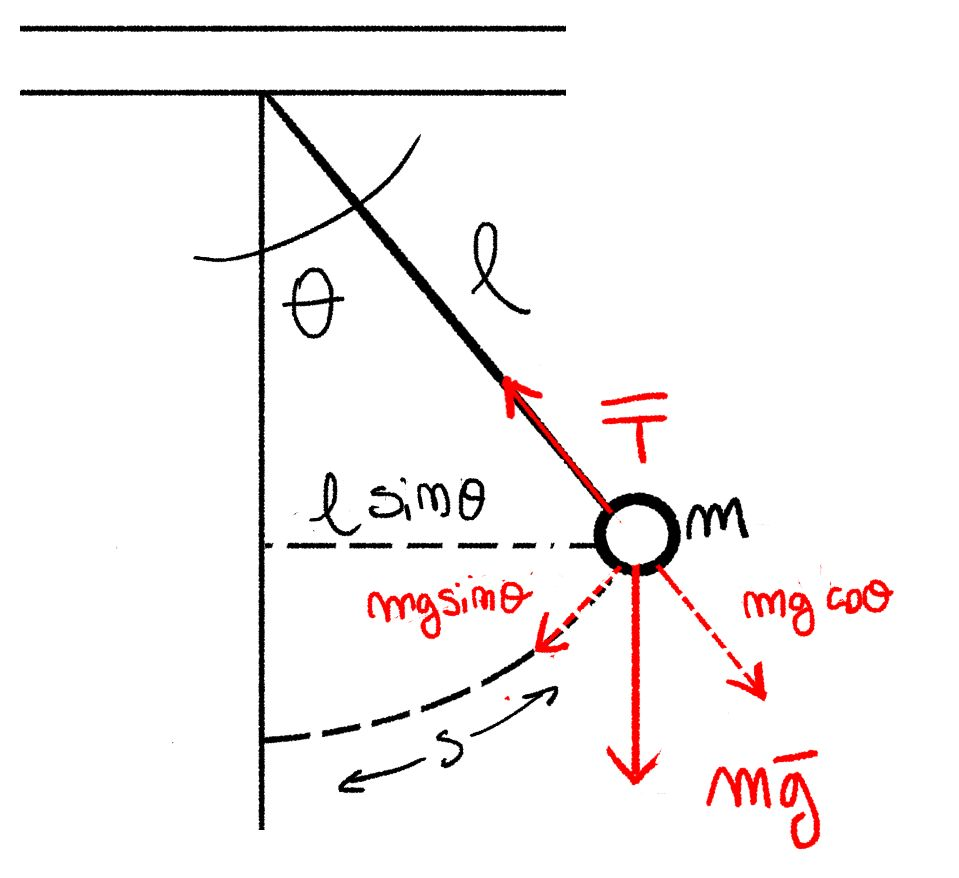
\includegraphics[height=1.7in]{images3/pendulum.jpg}
\end{center}
\pause

   \column{2.5in}


Ecuation of motion?
\pause
\begin{eqnarray}
T-mgcos\theta&=&ma_c\\
-mgsin\theta&=&ma_T
\label{eq:3}
\end{eqnarray}
\pause
We are going to use the equation \ref{eq:3}:


\begin{equation}
a_T+gsin\theta=0
\end{equation}

   \end{columns}






\end{frame}



%%%%%%%%%%%%%%%%%%%%%%%%%%%%%%%%%%%%%%%%%%%%%%%%%%%%%%%%%%%%%%%

\begin{frame}
\frametitle{The Simple Pendulum}

Then we have to solve  $a_T+gsin\theta=0$, for $\theta$. 
\vspace{3mm}
\pause

Note that the acceleration is related with $\theta$:
\pause

\begin{eqnarray*}
a_T&=&\ell \alpha\\
\alpha&=&\frac{d^2\theta}{dt^2}
\end{eqnarray*}

\pause

Then, we can write the equation for $\theta$ as,
\pause

\begin{equation}
\ell \frac{d^2\theta}{dt^2}+gsin\theta=0
\label{eq:4}
\end{equation}


\end{frame}

%%%%%%%%%%%%%%%%%%%%%%%%%%%%%%%%%%%%%%%%%%%%%%%%%%%%%%%%%%%%%%%

\begin{frame}
\frametitle{The Simple Pendulum}

The equation \ref{eq:4} is not exactly the equation of a simple harmonic oscillator, but we can make the following approximation for small angles:

\begin{equation*}
sin\theta\sim \theta
\end{equation*}

where $\theta$ is measured in radians.


\end{frame}
%%%%%%%%%%%%%%%%%%%%%%%%%%%%%%%%%%%%%%%%%%%%%%%%%%%%%%%%%%%%%%%

\begin{frame}
\frametitle{The Simple Pendulum}


Note that:

\begin{eqnarray*}
sin\theta&=&\sum \frac{(-1)^n}{(2n+1)!}\theta^{2n+1}\\
&=&\theta-\frac{\theta^3}{3!}+\frac{ \theta^5}{5!}-...
\end{eqnarray*}
 
if $\theta \leq 15^{\circ}\rightarrow sin\theta\sim \theta$

\begin{eqnarray*}
sin(15^{\circ})&=&0.2588190451\\
15^{\circ}&=&0.26179938779~rad
\end{eqnarray*}

\end{frame}

%%%%%%%%%%%%%%%%%%%%%%%%%%%%%%%%%%%%%%%%%%%%%%%%%%%%%%%%%%%%%%%

\begin{frame}
\frametitle{The Simple Pendulum}

Then, for small angles,
\pause

\begin{equation}
\ell \frac{d^2\theta}{dt^2}+g\theta=0
\label{eq:5}
\end{equation}
\pause

The solution of this equation is:
\pause

\begin{equation}
\theta (t)=\theta_0cos(\omega t)
\label{eq:6}
\end{equation}
\pause

were 
\pause

\begin{equation}
\omega=\sqrt{\frac{g}{\ell}}
\label{eq:6}
\end{equation}
\pause

and  we consider that at $t=0$, the initial angle is $\theta_0$ and the velocity is $v_0=0$.

\end{frame}



%%%%%%%%%%%%%%%%%%%%%%%%%%%%%%%%%%%%%%%%%%%%%%%%%%%%%%%%%%%%%%%

\begin{frame}
\frametitle{The Simple Pendulum}

The period of the motion is,

\begin{equation}
T=\frac{2\pi}{\omega}=2\pi\sqrt{\frac{\ell}{g}}
\end{equation}
\pause

\vspace{3mm}
We can measure $g$ using a pendulum!
\vspace{3mm}

\pause
\textbf{Question}: If a simple pendulum is taken from sea level to the top of a high mountain
and started at the same angle of 5°, it would oscillate at the top of the mountain
(a) slightly slower, (b) slightly faster, (c) at exactly the same frequency, (d)  none of these.

\end{frame}


%%%%%%%%%%%%%%%%%%%%%%%%%%%%%%%%%%%%%%%%%%%%%%%%%%%%%%%%%%%%%%%

\begin{frame}
\frametitle{The Physical Pendulum}

The term physical pendulum refers to any real extended object which oscillates back
and forth.


   \begin{columns}[c]
   \column{2in}  % slides are 3in high by 5in wide
  

  \begin{center}
  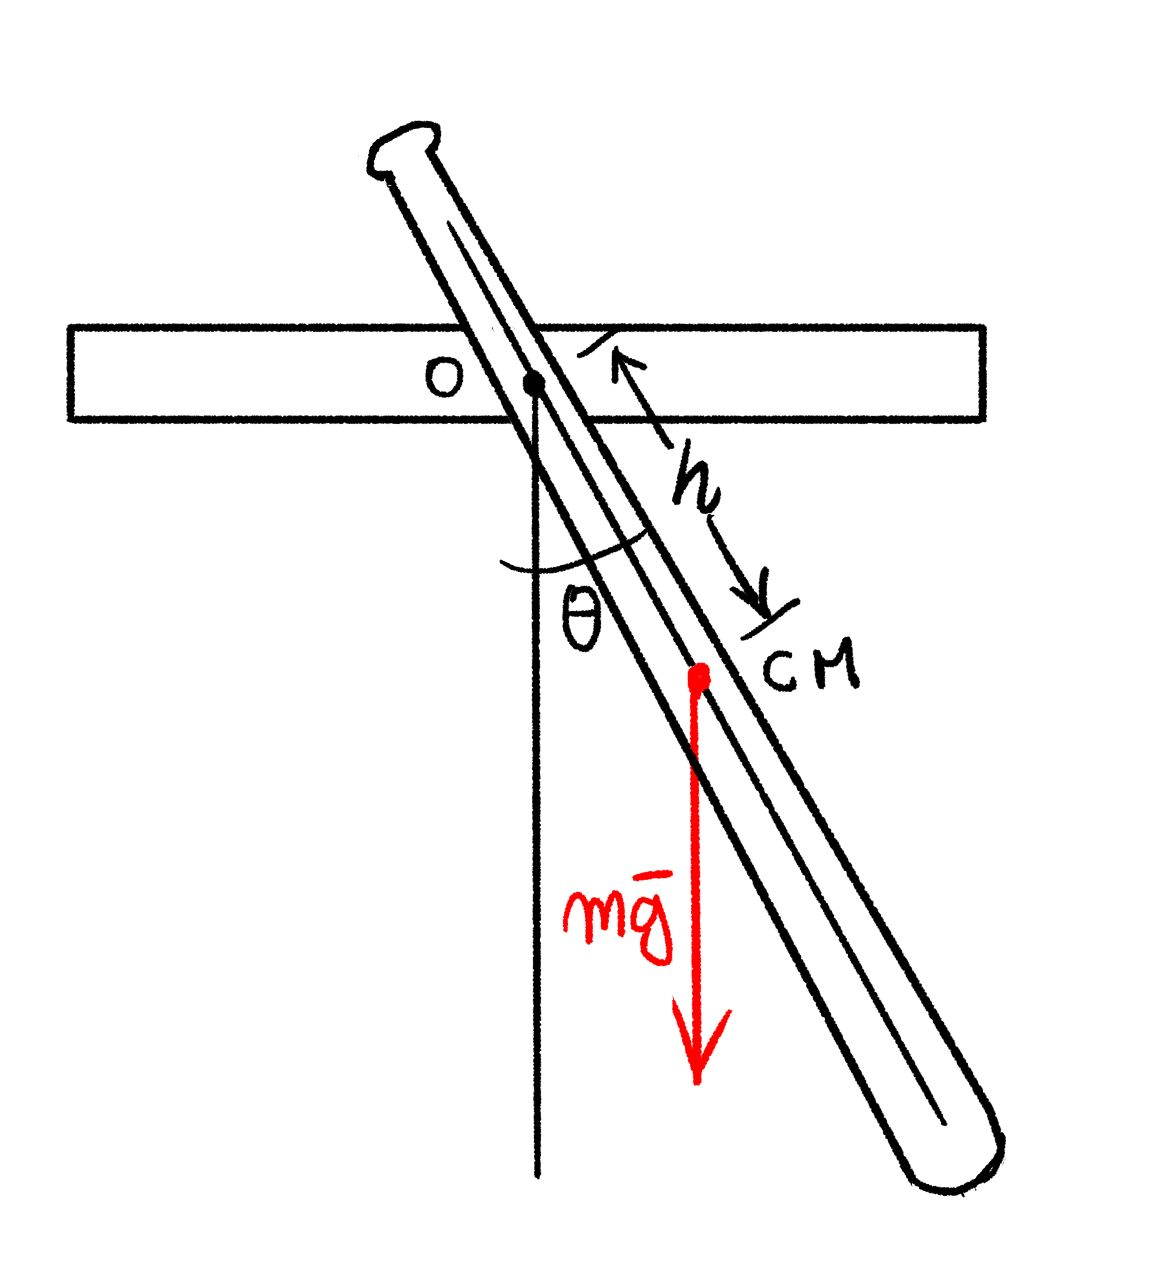
\includegraphics[height=1.7in]{images3/physical_pendulum.jpg}
\end{center}


\pause
   \column{2.8in}

\begin{eqnarray*}
torque\rightarrow N&=&-hmg~sin\theta \\
\pause
\rightarrow I\alpha&=&-hmg~sin\theta \\
\\
\pause
\rightarrow I\frac{d^2\theta}{dt^2}&=&-hmg~sin\theta \\
\end{eqnarray*}
\pause

The, the equation for small angles is,

\pause

\begin{equation}
\frac{d^2\theta}{dt^2}+\frac{hmg}{I}\theta=0
\label{eq:9}
\end{equation}

   \end{columns}



\end{frame}




%%%%%%%%%%%%%%%%%%%%%%%%%%%%%%%%%%%%%%%%%%%%%%%%%%%%%%%%%%%%%%%

\begin{frame}
\frametitle{The Physical Pendulum}

The solution of the equation \ref{eq:9} is:

\begin{equation*}
\theta(t)=\theta_0 cos(\omega t)
\end{equation*}
\pause
where,

\begin{equation}
\omega= \sqrt{\frac{hmg}{I}}
\end{equation}
\pause
where the velocity at $t=0$ is $v_0=0$ and the angle is $\theta(t=0)=\theta_0$.
\pause
The period of the oscillations is,
\pause
\begin{equation}
T= 2\pi \sqrt{\frac{I}{hmg}}
\end{equation}
\pause
We can measure the inertia moment using a pendulum motion.

\end{frame}


%%%%%%%%%%%%%%%%%%%%%%%%%%%%%%%%%%%%%%%%%%%%%%%%%%%%%%%%%%%%%%%

\begin{frame}
\frametitle{Summarizing...}

A restoring force gives place to an simple harmonic motion.

\begin{equation*}
F=-kx\rightarrow\frac{d^2x}{dt^2}+\frac{k}{m}x=0
\end{equation*}
\pause
The solution is...
\vspace{3mm}

\pause

\begin{equation*}
x(t)=Acos(\omega t + \phi)=A'cos(\omega t)+B' sin(\omega t)
\end{equation*}

\pause

\begin{equation*}
\omega=\sqrt{\frac{k}{m}}
\end{equation*}

\pause

and the other constant depends on the intitial conditions.

\end{frame}
%%%%%%%%%%%%%%%%%%%%%%%%%%%%%%%%%%%%%%%%%%%%%%%%%%%%%%%%%%%%%%%

\begin{frame}
\frametitle{Summarizing...}

All the following systems have simple harmonic motion..


  \begin{center}
  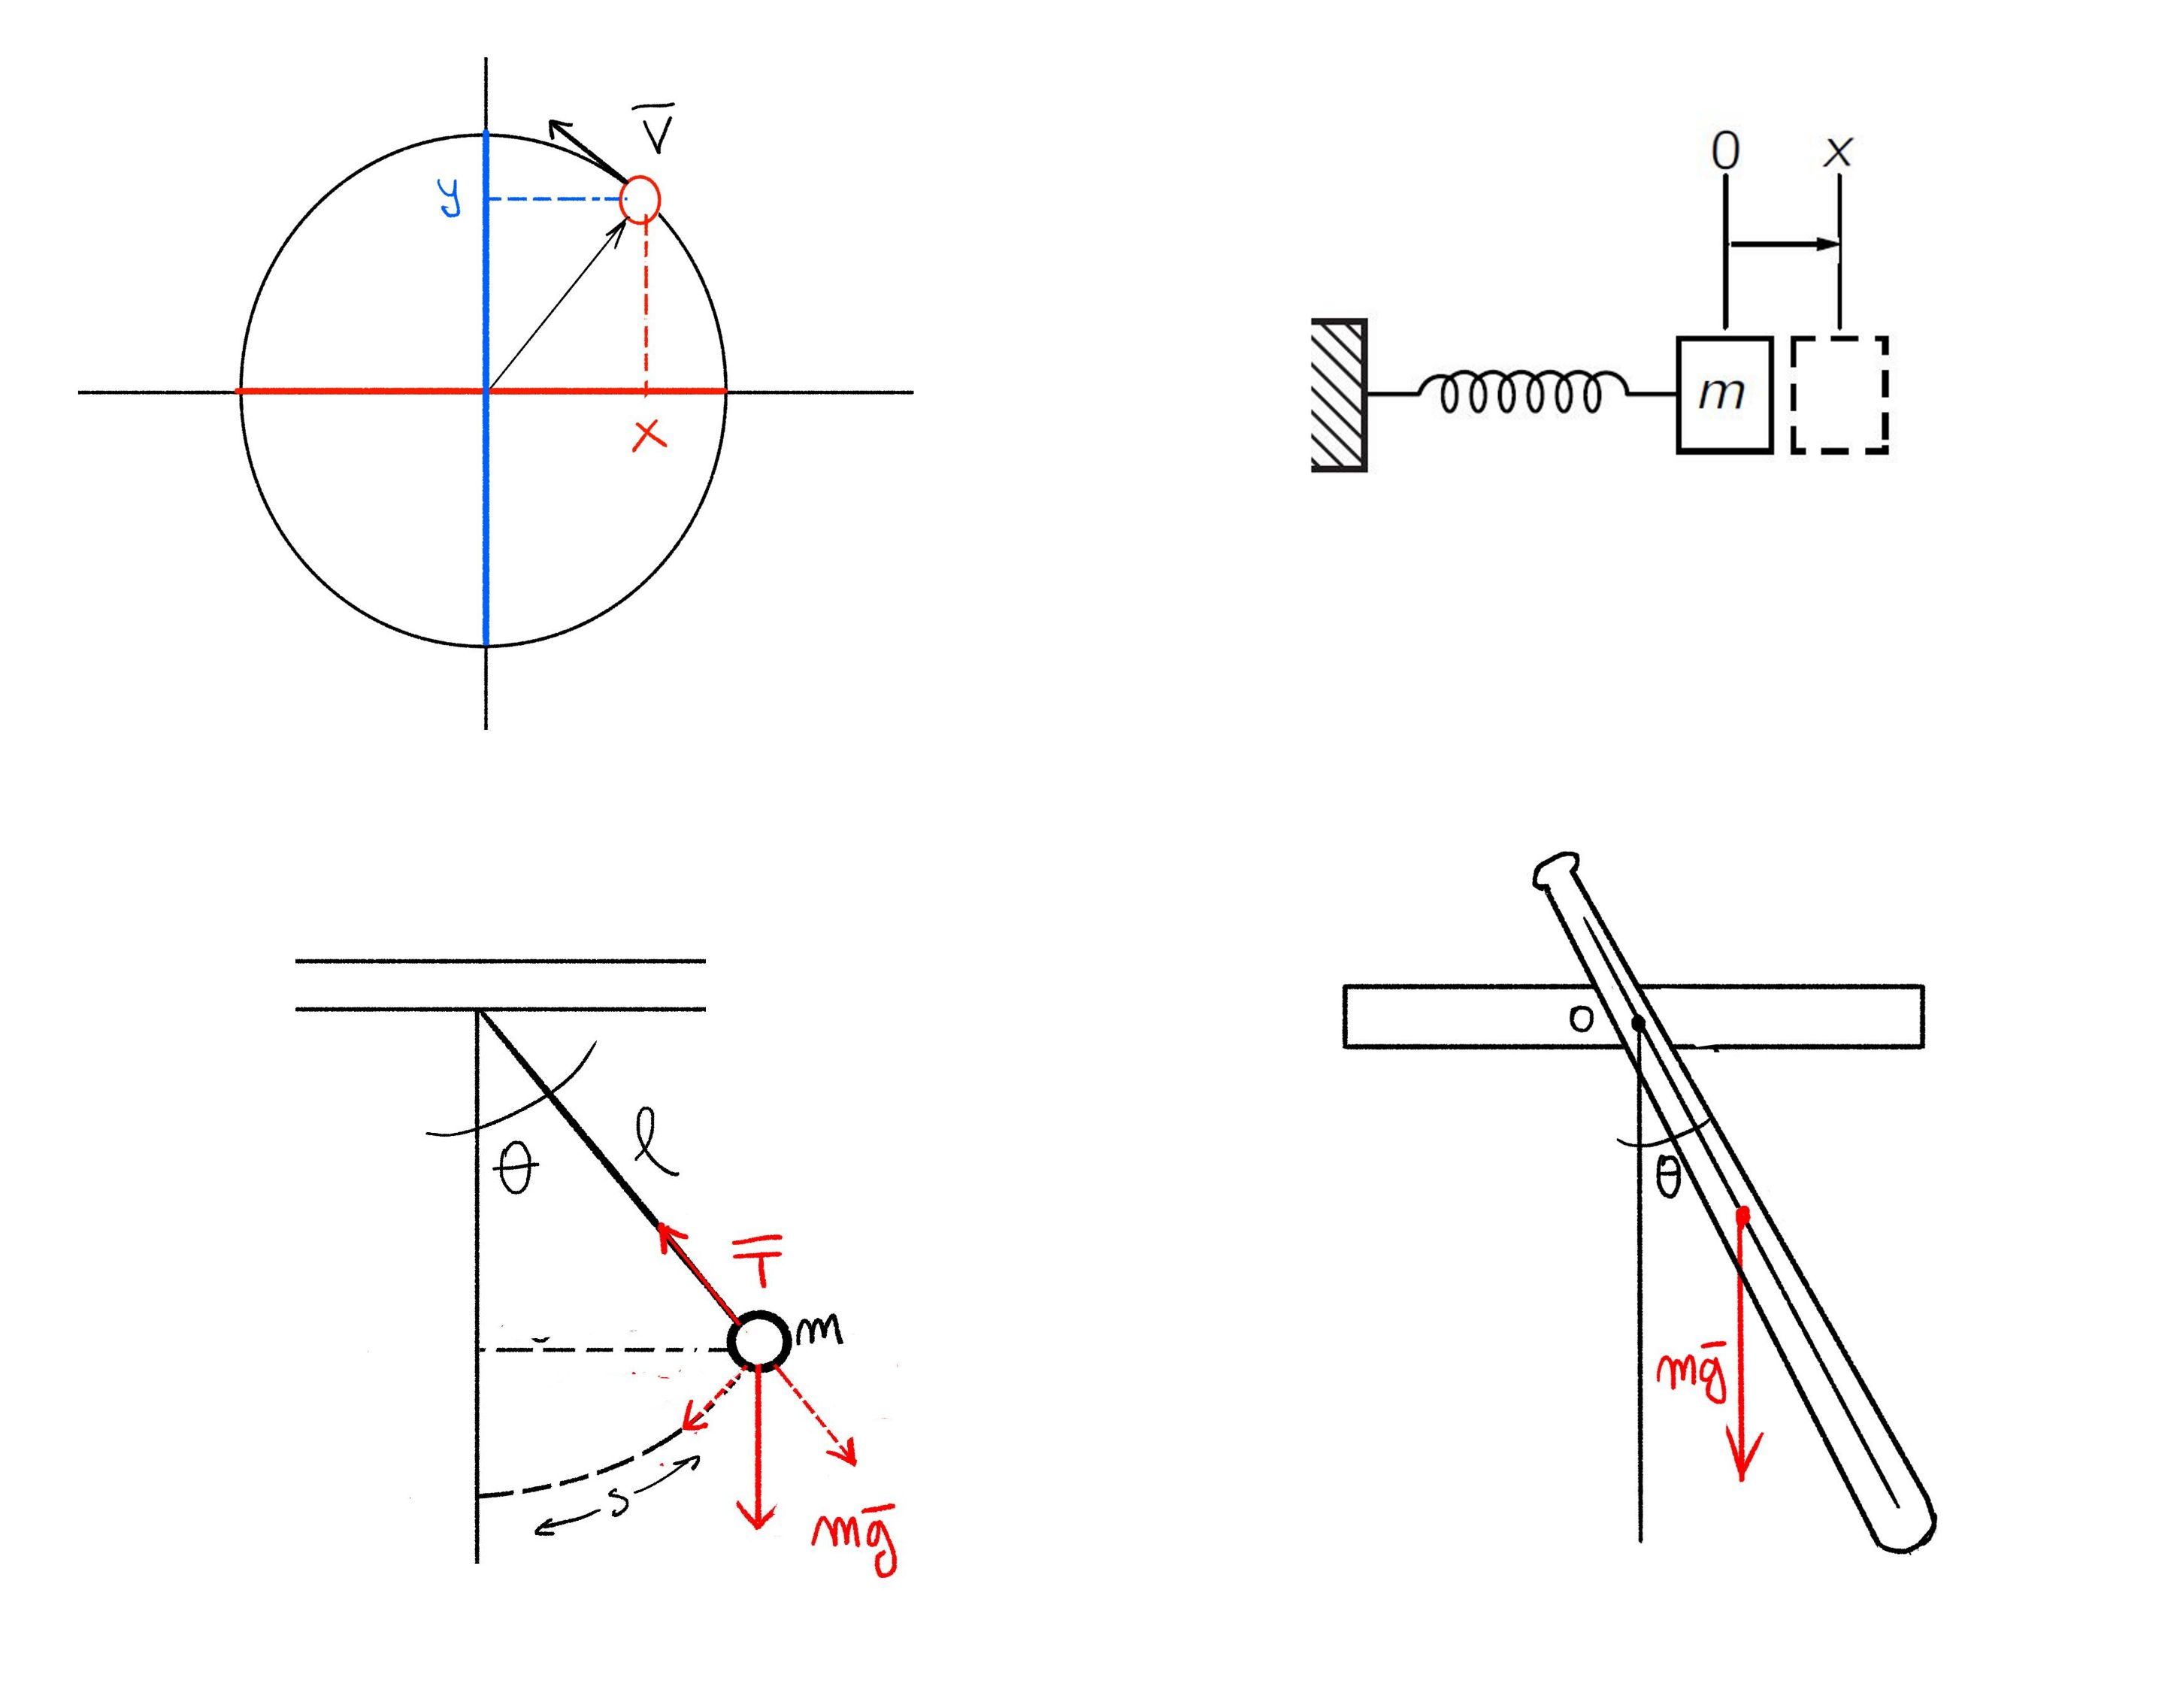
\includegraphics[height=2.6in]{images3/summarizing2.jpg}
\end{center}


\end{frame}





%%%%%%%%%%%%%%%%%%%%%%%%%%%%%%%%%%%%%%%%%%%%%%%%%%%%%%%%%%%%%%%

\begin{frame}
\frametitle{Damped Harmonic Motion}
\pause
Drag force
 due to the viscosity of the air:

 \pause

\begin{equation*}
\boxed{F_d=-bv}
\end{equation*}
\pause

Then,

\begin{equation*}
ma=-kx\textcolor{mypink1}{-bv}
\end{equation*}

\pause


\begin{equation}
\rightarrow \boxed{\frac{d^2x}{dt^2}+\frac{b}{m}\frac{dx}{dt}+\frac{k}{m}x=0}
\label{eq:10}
\end{equation}


\end{frame}


%%%%%%%%%%%%%%%%%%%%%%%%%%%%%%%%%%%%%%%%%%%%%%%%%%%%%%%%%%%%%%%

\begin{frame}
\frametitle{Damped Harmonic Motion}

The drag force depends on $v$, $\pause\rightarrow$ it is  not conservative $\pause\rightarrow$ the energy is lost $\pause\rightarrow$ the amplitude  decreases
\pause

\vspace{3mm}

\pause

Trial solution:

\pause

\begin{equation*}
x(t)=A\textcolor{mypink1}{e^{-\gamma t}}cos\omega' t
\end{equation*}

\pause

What are $\gamma$ and $\omega'$?
\vspace{3mm}

\pause
 To find them, we have to introduce the solution in the equation (\ref{eq:10})...


\end{frame}






%%%%%%%%%%%%%%%%%%%%%%%%%%%%%%%%%%%%%%%%%%%%%%%%%%%%%%%%%%%%%%%

\begin{frame}
\frametitle{Damped Harmonic Motion}

We find...

\begin{equation}
\gamma=\frac{b}{2m}
\end{equation}

\begin{equation}
\omega'=\sqrt{\frac{k}{m}-\frac{b^2}{4m^2}}
\end{equation}

\pause

We can add a phase constant, in this case we considered $\phi=0$, then 

\begin{equation*}
v_0=0,~A=x_0
\end{equation*}

\end{frame}
%%%%%%%%%%%%%%%%%%%%%%%%%%%%%%%%%%%%%%%%%%%%%%%%%%%%%%%%%%%%%%%

\begin{frame}
\frametitle{Damped Harmonic Motion}

The frequency is,
\pause
\begin{equation}
f'=\frac{\omega'}{2\pi}=\frac{1}{2\pi}\sqrt{\frac{k}{m}\textcolor{mypink1}{-\frac{b^2}{4m^2}}}
\end{equation}
\pause

\vspace{3mm}

\pause
So, the frequency is lower, and the period longer.
\vspace{3mm}

\pause
Limit for $b$:
\pause

\begin{equation}
b^2<4mk
\end{equation}

\end{frame}
%%%%%%%%%%%%%%%%%%%%%%%%%%%%%%%%%%%%%%%%%%%%%%%%%%%%%%%%%%%%%%%

\begin{frame}
  \frametitle{Damped Harmonic Motion}
  
When $b^2>4mk$, the solution is:
\vspace{3mm}

\begin{equation}
  x=C_1 e^{-a_1 t}+C_2 e^{-a_2 t}
\end{equation}
\vspace{3mm}

\pause

$a_1~ and~ a_2 ~\pause \rightarrow~ \textcolor{mypink1}{depend~ on~ m,~ k,~ and~ b}$
\\
\vspace{3mm}
$\pause C_1~ and~ C_2 ~\pause \textcolor{mypink1}{\rightarrow~ depend~ on~the~ intitial~ conditions}$

  \end{frame}
  


%%%%%%%%%%%%%%%%%%%%%%%%%%%%%%%%%%%%%%%%%%%%%%%%%%%%%%%%%%%%%%%

\begin{frame}
\frametitle{Damped Harmonic Motion}


Then, the solutions look like this...

\pause
  \begin{center}
  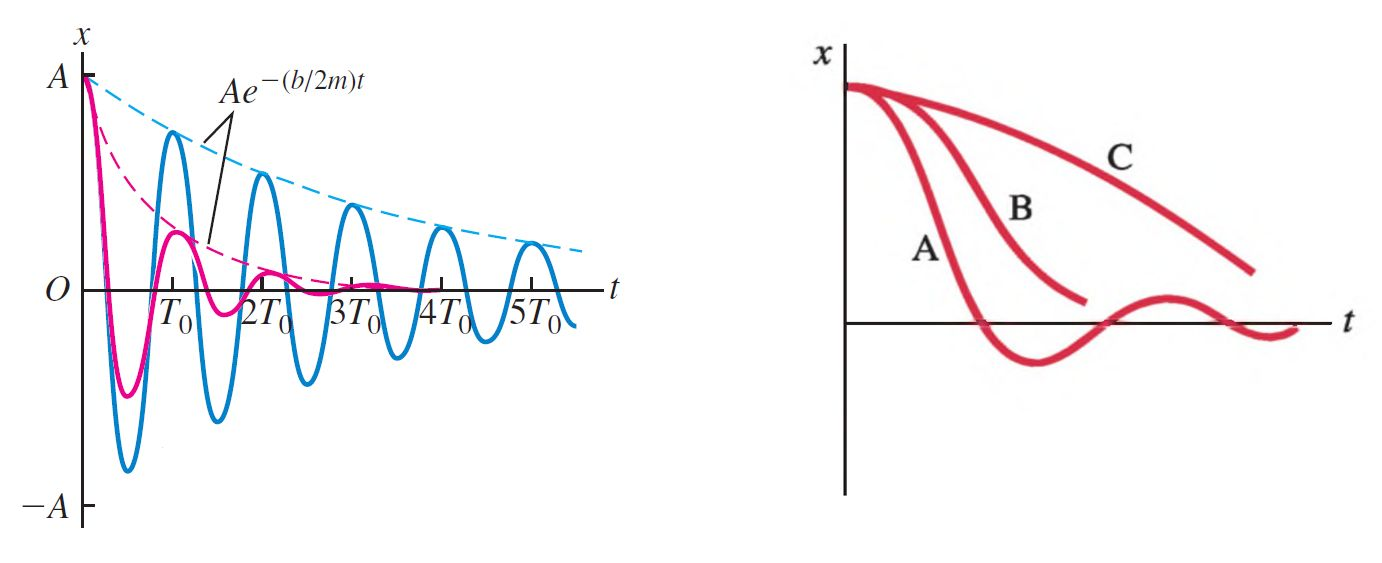
\includegraphics[height=1.8in]{images3/dampling3.jpg}
\end{center}




\end{frame}


%%%%%%%%%%%%%%%%%%%%%%%%%%%%%%%%%%%%%%%%%%%%%%%%%%%%%%%%%%%%%%%

\begin{frame}
\frametitle{Damped Harmonic Motion}

Then, the solutions look like this...


  \begin{center}
  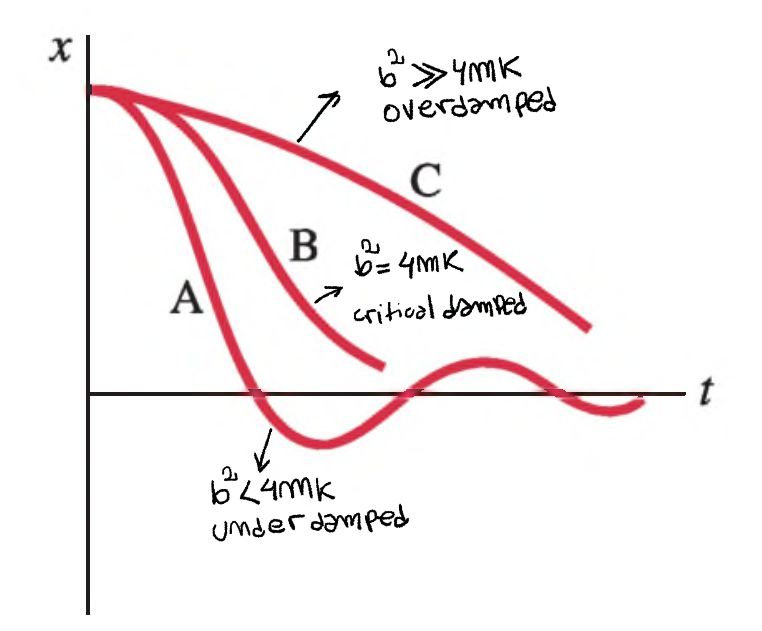
\includegraphics[height=2.5in]{images3/dampling2b.jpg}
\end{center}




\end{frame}

%%%%%%%%%%%%%%%%%%%%%%%%%%%%%%%%%%%%%%%%%%%%%%%%%%%%%%%%%%%%%%%

\begin{frame}
  \frametitle{Damped Harmonic Motion}
  
  \textcolor{mypink1}{Energy in damped Oscillations}
  
  \pause

  \begin{equation*}
    \frac{dE}{dt}   \pause =mv_x\frac{dv_x}{dt}+kx\frac{dx}{dt}
  \end{equation*}
  \pause

  \begin{equation*}
    \rightarrow \frac{dE}{dt}   \pause =v_x(ma_x+kx)
  \end{equation*}
  

  \pause

  \begin{equation*}
    \rightarrow \frac{dE}{dt}   \pause =v_x(-b v_x)\pause =-b v_x^2
  \end{equation*}

  \end{frame}
  



%%%%%%%%%%%%%%%%%%%%%%%%%%%%%%%%%%%%%%%%%%%%%%%%%%%%%%%%%%%%%%%

\begin{frame}
\frametitle{Example 1}



A simple pendulum has a length of $\ell$. It is set swinging with small-amplitude oscillations.
After a time $\Delta t$, the amplitude is only 50$\%$ of what it was initially, (a) What is
the value of $\gamma$ for the motion? (b) By what factor does the difference between the frequencies, $f-f'$, differ
from $f$, the undamped frequency?



\end{frame}

%%%%%%%%%%%%%%%%%%%%%%%%%%%%%%%%%%%%%%%%%%%%%%%%%%%%%%%%%%%%%%%

\begin{frame}
\frametitle{Test your understanding...}


\begin{enumerate}
\item Is the acceleration of a simple harmonic oscillator ever zero? If so, where?
\pause
\item For a simple harmonic oscillator, when (if ever) are the
displacement and velocity vectors in the same direction?
When are the displacement and acceleration vectors in the
same direction?
\pause
\item Two equal masses are attached to separate identical springs
next to one another. One mass is pulled so its spring
stretches $20~cm$ and the other is pulled so its spring stretches
only $10~cm$. The masses are released simultaneously. Which
mass reaches the equilibrium point first?
\pause
\item A thin uniform rod of mass m is suspended from one end
and oscillates with a frequency $f$ . If a small sphere of mass
$2m$ is attached to the other end, does the frequency increase
or decrease? Explain.

\end{enumerate}



\end{frame}

%%%%%%%%%%%%%%%%%%%%%%%%%%%%%%%%%%%%%%%%%%%%%%%%%%%%%%%%%%%%%%%

\begin{frame}
\frametitle{ Forced oscillations; Resonance}


Adding an  external force 

\pause

 \begin{equation}
F_{ext}=F_0cos\omega t
\end{equation}

\pause

$\omega_0\neq\sqrt{\frac{k}{m}}$ (natural frequency of the spring).

\vspace{5mm}

\textcolor{mypink1}{If the frequency of the force is near the natural frequency of the spring, the amplitude of the motion can become very large. 
This effect is known as \textbf{resonance} and the natural frequency of
the system is $f_0$, the \textbf{resonant frequency}. }

\end{frame}



%%%%%%%%%%%%%%%%%%%%%%%%%%%%%%%%%%%%%%%%%%%%%%%%%%%%%%%%%%%%%%%

\begin{frame}
\frametitle{ Forced oscillations; Resonance}


Equation of motion:

\vspace{3mm}
 \begin{equation}
ma=-kx-bv+\textcolor{mypink1}{F_0cos\omega t}
\end{equation}
\vspace{3mm}
\pause


 \begin{equation}
\rightarrow \frac{d^2x}{dt^2}+b\frac{dx}{dt}+kx=F_0cos\omega t
\end{equation}
\pause


\vspace{3mm}
The trial solution is this time,
\pause


 \begin{equation}
x(t)=A_0sin(\omega t +\phi_0)
\end{equation}


\end{frame}




%%%%%%%%%%%%%%%%%%%%%%%%%%%%%%%%%%%%%%%%%%%%%%%%%%%%%%%%%%%%%%%

\begin{frame}
\frametitle{ Forced oscillations; Resonance}


We can find $A_0$ and $\phi_0$ by direct substitution,

\pause
   \begin{columns}[c]
   \column{2in}  % slides are 3in high by 5in wide
  

 \begin{equation*}
A_0=\frac{F_0}{m\sqrt{(\omega^2-\omega^2_0)^2+b^2\omega^2/m^2}}
\end{equation*}
\pause

and


 \begin{equation*}
\phi_0=tan^{-1}\frac{\omega^2_0-\omega^2}{\omega(b/m)}
\end{equation*}

   \column{2in}

\pause

  \begin{center}
  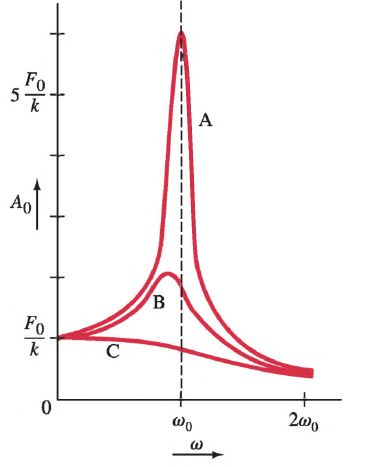
\includegraphics[height=2.2in]{images3/resonance.jpg}
\end{center}


   \end{columns}

   
\end{frame}














%%%%%%%%%%%%%%%%%%%%%%%%%%%%%%%%%%%%%%%%%%%%%%%%%%%%%%%%%%%%%%%
 \end{document}
%%%%%%%%%%%%%%%%%%%%%%%%%%%%%%%%%%%%%%%%%%%%%%%%%%%%%%%%%%%%%%%